\documentclass[10pt,a4paper]{article}
\usepackage[utf8]{inputenc}
\usepackage{amsmath}
\usepackage{amsfonts}
\usepackage{amssymb}
\usepackage[margin=3cm]{geometry}
\usepackage{xspace}
\usepackage{enumerate}
\usepackage{graphicx}
\usepackage{hyperref}
\begin{document}


\begin{center}
{\huge Ethereum Difficulty Updates}

{\small Aeron Buchanan, version 2}
\end{center} 

\section*{Conclusion}
Ethereum difficulty would be more stable if either 1) updated very much less often than every block, and/or 2) updated with a more sophisticated formula. The nature of proof-of-work means block-times vary hugely: with a target block-time of 1, the raw stats give $\sigma>0.9$. Without any updates, an optimized difficulty setting gives a running 500-block-time average $^{500}\sigma<0.05$. This can be matched with sophisticated enough update strategies, such as a PID controller. Using the update strategy of the white paper V2 $^{500}\sigma\approx0.1$. Demonstrations of stability are given below. I recommend the strategy employed by bitcoin, which compromises simplicity with an ability to stably track changes in network processing power. It should be noted that the difficulty has to be increased whenever more nodes join the network, whether they are more powerful than the average node or not.

\section*{Introduction}

Proof-of-Work (PoW) is an unfortunate necessity for dealing with ``infinite virtual node'' and ``spam'' attacks in a consensus based event log (commonly referred to as the block-chain). Anyone can add events to the shared log and so forks and branches will develop as additions are accepted by some and ignored by others. Additions can be ignored because someone deems them unacceptable or because the proposer is on a far flung corner of the network and delays in communications mean that the consensus has moved on too far by the time enough people get notified of them. When you come to read the log or make an addition, which event log do you take as the master? Being a consensus, it must be the log with the most votes. However, without PoW it would be trivial to create a large number of nodes to vote for (verify) a thief's log in which they erased an entry that they had used to pay someone, thus allowing them to spend that money a second time. In a pure identity-based voting system, the person with the most resources can win control of the system, as they can out-vote an uncoordinated honest majority. Furthermore, if it costs nothing to add events then the system can be spammed by attackers and rendered useless. Introducing PoW solves all these problems. With PoW, every one of the $N$ nodes gets to make many (quick, but non-negligible-time) attempts to add events to their favored log (and thus vote for it), each with a low chance of success. It provides a better solution to the voting problem, because on average, everyone gets roughly a $\frac{m}{N}$ chance of voting for a particular event log with $m$ being the multiple of the average node resources a particular node has. It also solves the spamming and network-delay problems by making it take, on average, an appreciable amount of time to add events to the log. However, as the available processing power changes, the average number of attempts that can be made per time will change, and so the effectiveness of the PoW will change. If processing power increases (faster nodes or more of them), the average time taken will decrease, reducing the effectiveness of the PoW, and vice versa. As such, the difficulty of a PoW attempt must be adjusted. Here, I briefly discuss update strategies.

\newpage

\section*{Strategy}

To maintain a target block-time addition rate of one block per minute (or any target time) the difficulty of the atomic mining operation will have to be updated over time. Vitalik's updated white paper suggests the following update strategy:

\begin{verbatim}
update := floor( difficulty(n-1) / 1000 )

if (timestamp(n-1) - timestamp(n-500)) / 500 > 60
    difficulty(n) := difficulty(n-1) - update
else
    difficulty(n) := difficulty(n-1) + update
\end{verbatim}
where {\tt difficulty(n)} is the level for the current block and {\tt timestamp(n)} returns the time of the {\tt n}$^{th}$ block in seconds. The genesis block is {\tt n = 0} and all blocks before it are assumed to have the same {\tt timestamp} as the genesis block.

The averaging effectively adds lag to the system, so the result of an update is not seen until many blocks later. In the interim, the algorithm continues to change the difficulty in whatever the necessary direction. This leads to oscillations taking the 500-block average to $\pm 20\%$ when the underlying signal is steady-state (note that for clarity and ease of simulation, the probability of success, $p = \frac{1}{d}$, is used instead of the difficulty, $d$):

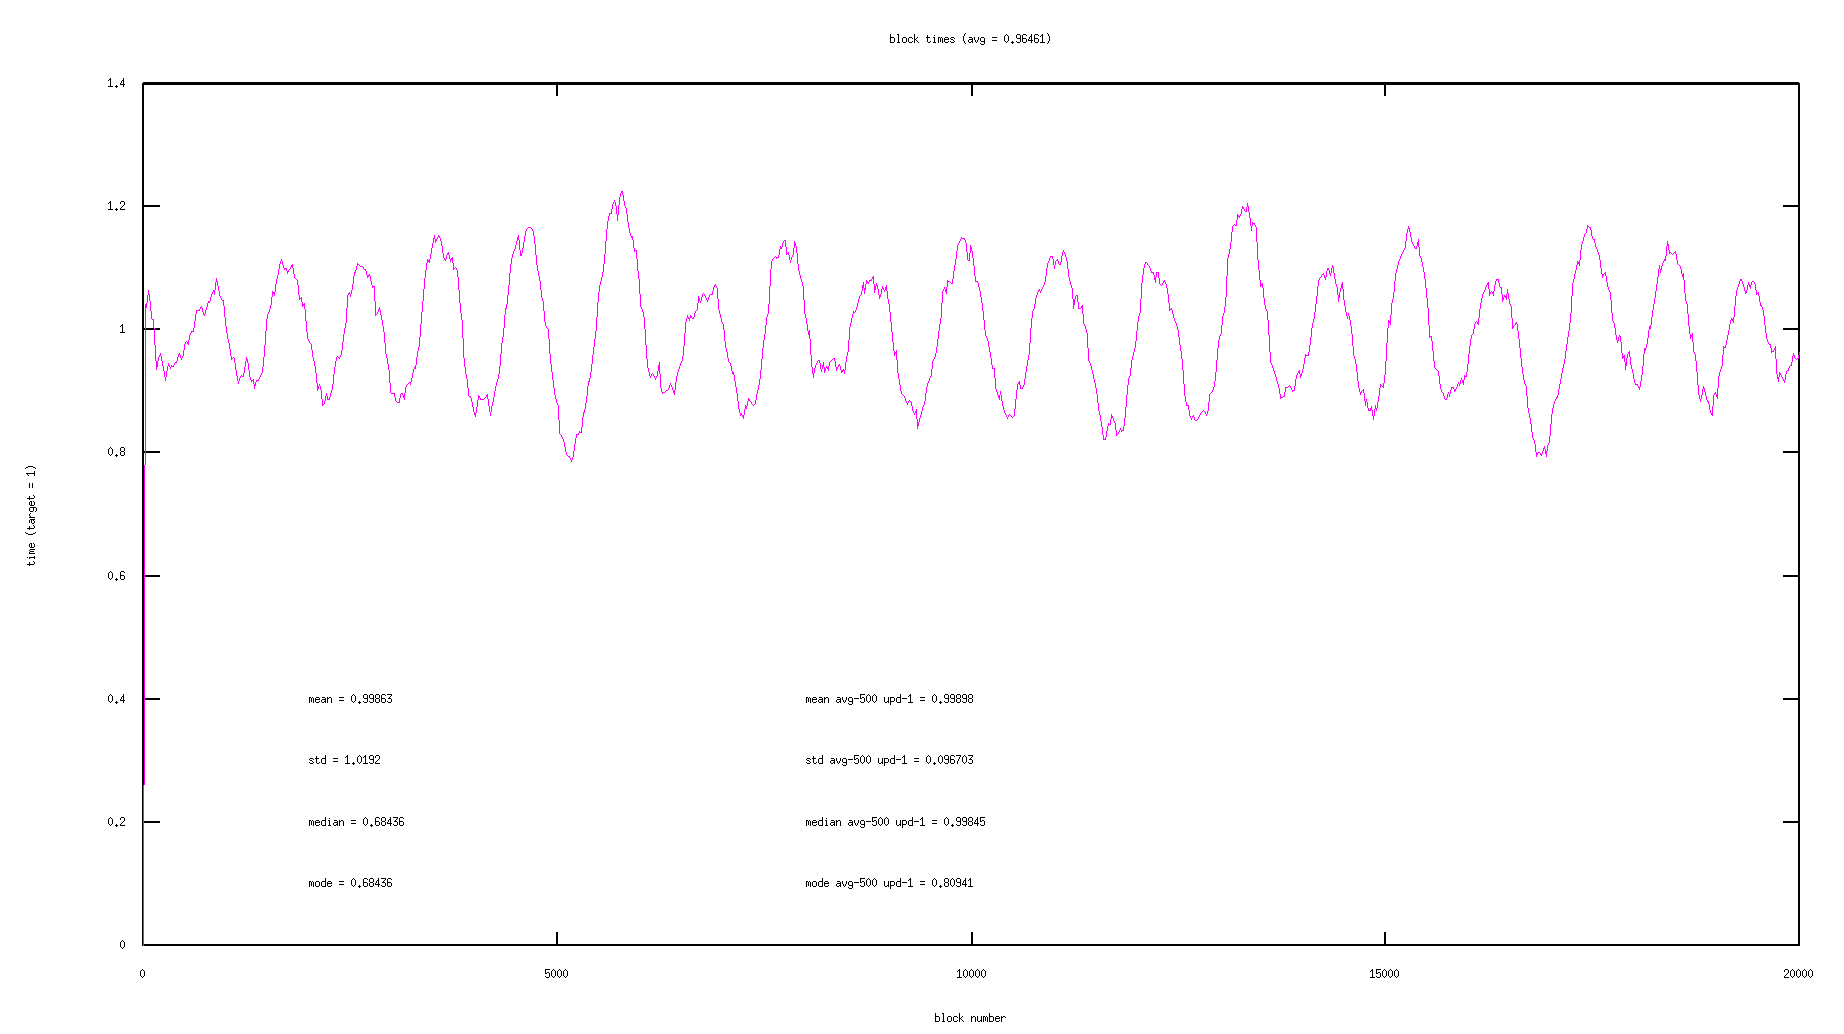
\includegraphics[width=13cm]{SimulationGraphs/simulation_avg-500_upd-1_.png}

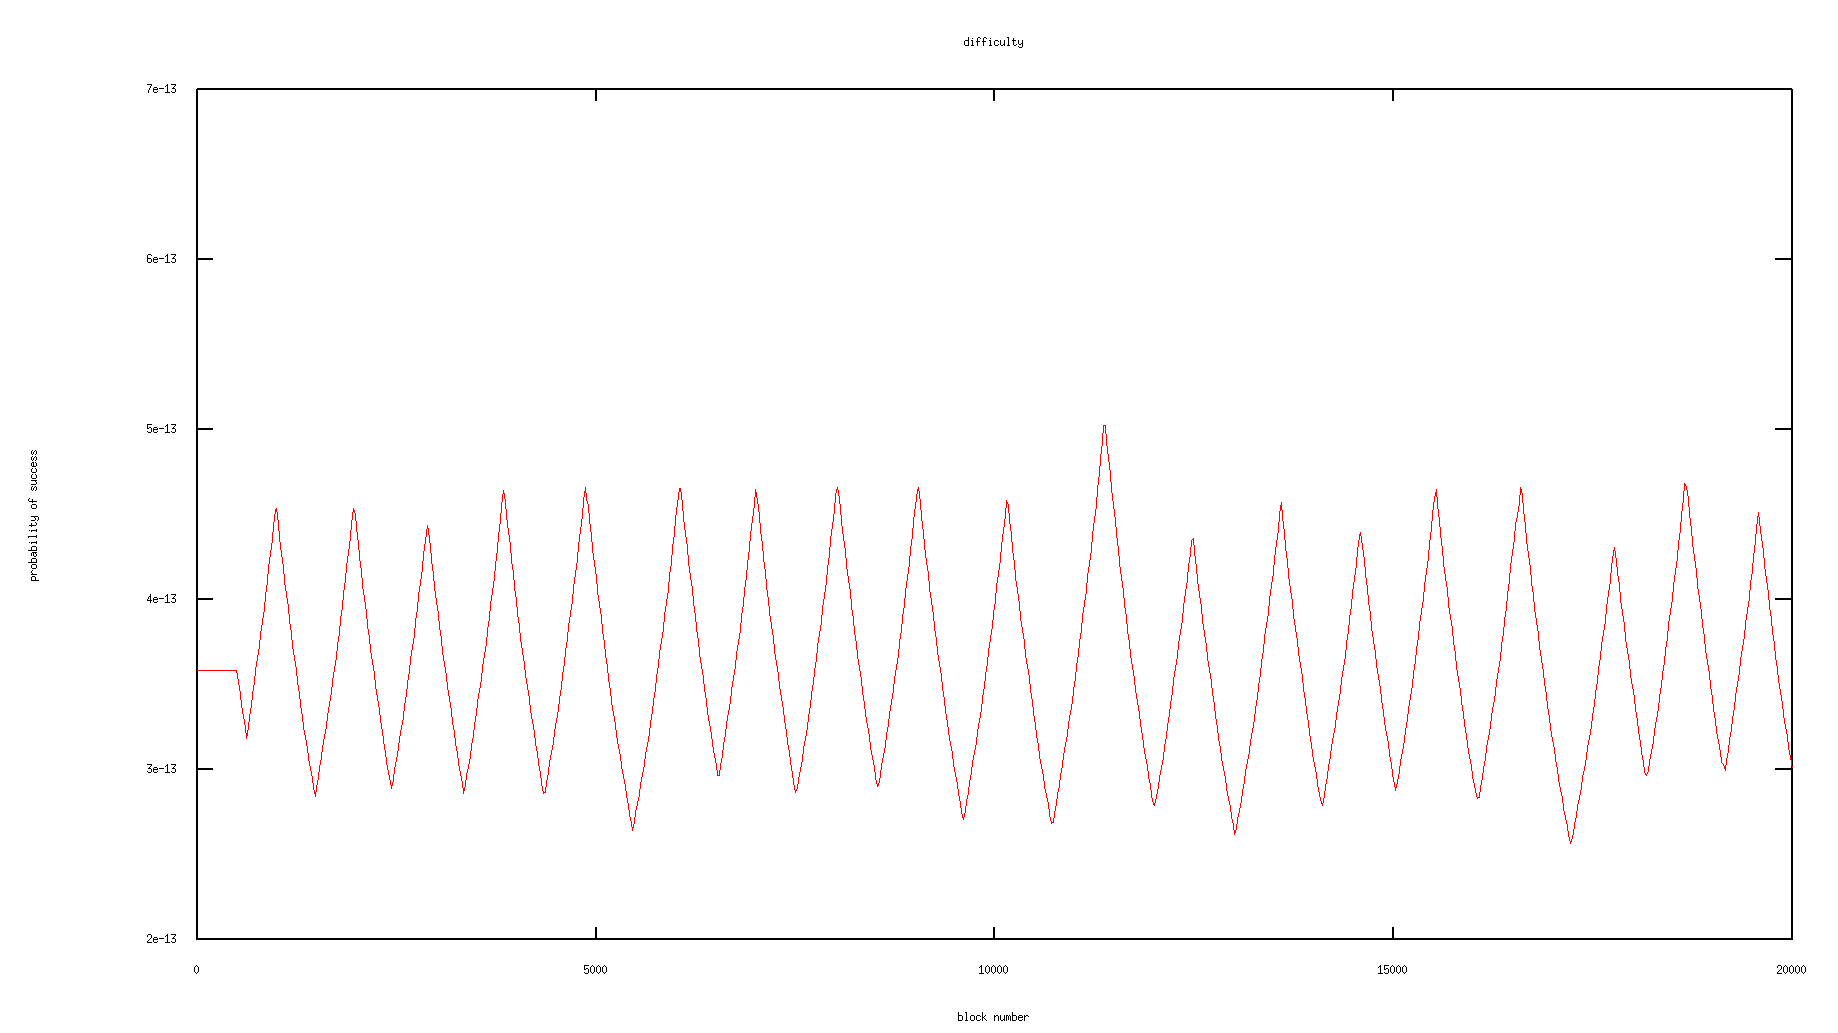
\includegraphics[width=13cm]{SimulationGraphs/simulation_avg-500_upd-1_diff.png}

This can be easily overcome by simply only updating every {\tt M} blocks:

\begin{verbatim}
if mod(n, M) = 0
{
    update := floor( difficulty(n-1) * k )

    if (timestamp(n-1) - timestamp(n-500)) / 500 > 60
        difficulty(n) := difficulty(n-1) - update
    else
        difficulty(n) := difficulty(n-1) + update
}
else
{
    difficulty(n) := difficulty(n-1)
}
\end{verbatim}
at the expense of responsiveness. However, the statistics of the mining nodes are not going to change dramatically in the order of 8 hours, so effective responsiveness is potentially adequate. The update {\tt k} must then be chosen to achieve a particular maximum update rate. The rate needs to be set high enough to be able to keep up with changes, but not so high as to create oscillatory behaviour when the mining power is not changing. Matching the first algorithm's ability to double in less than half a day, for example, is too much to update in one go:

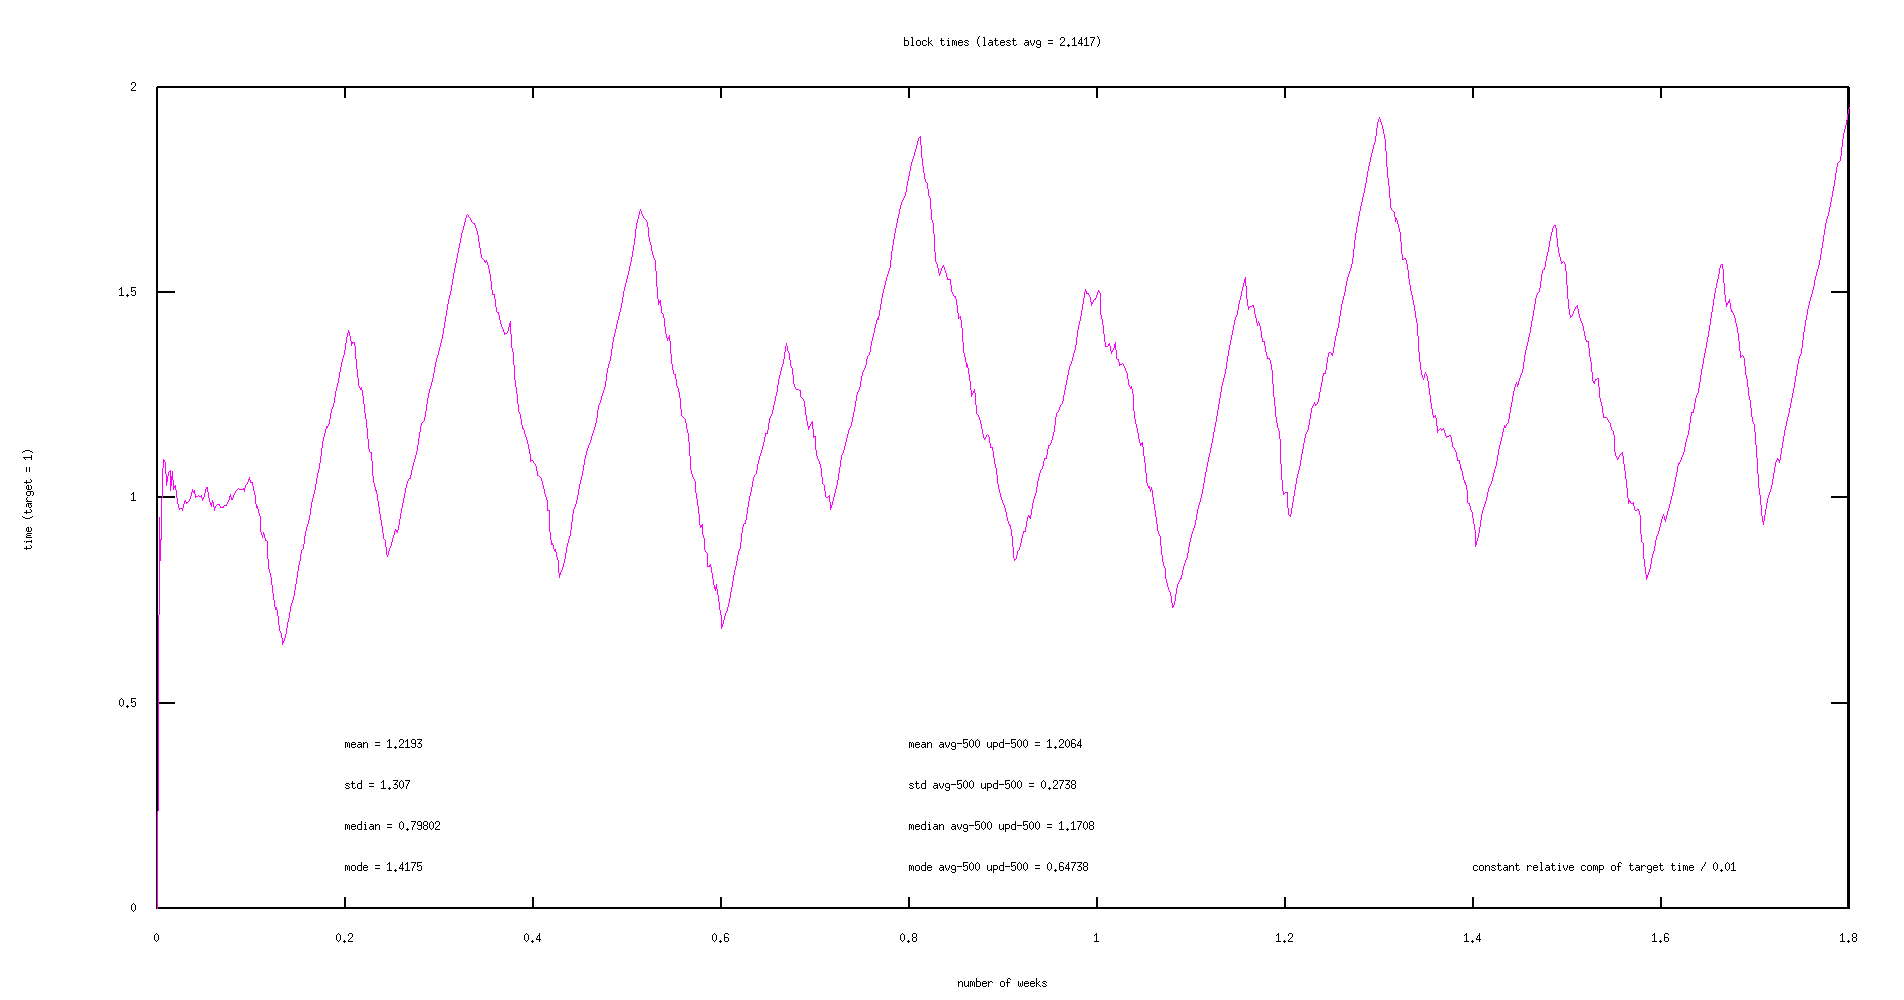
\includegraphics[width=14cm]{SimulationGraphs/simulation_avg-500_upd-500_p0-5.png}

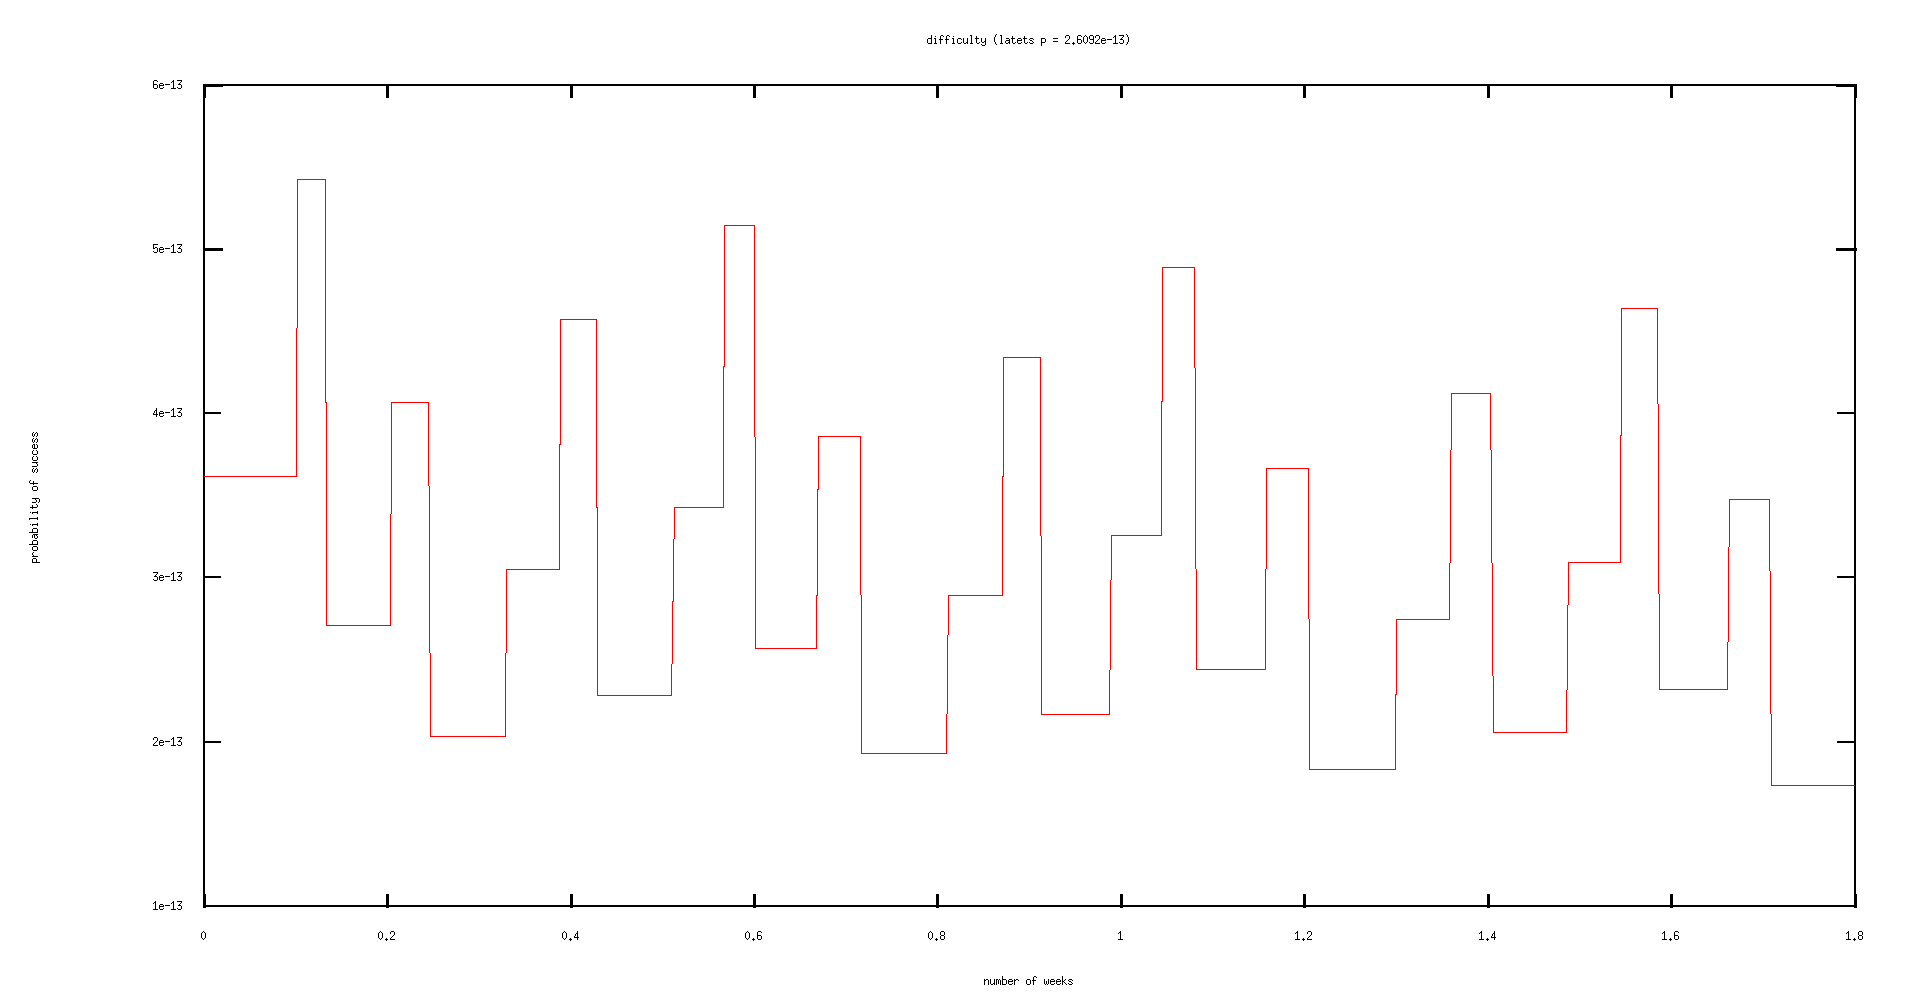
\includegraphics[width=14cm]{SimulationGraphs/simulation_avg-500_upd-500_p0-5_diff.png}

\newpage

Another approach is to use a proportional-style controller that updates by an amount proportional to the difference between the target and the actual (average) block-time, for example using the time difference in minutes divided by a constant (tuned here to 100):

\begin{verbatim}
if mod(n, M) = 0
{
    error := 1 - (timestamp(n-1) - timestamp(n-500)) / (500 * 60)
        
    update := 1 - error / 100

    difficulty(n) := difficulty(n-1) / update
}
else
{
    difficulty(n) := difficulty(n-1)
}
\end{verbatim}
Note: this is based on updating the probability proportionally.

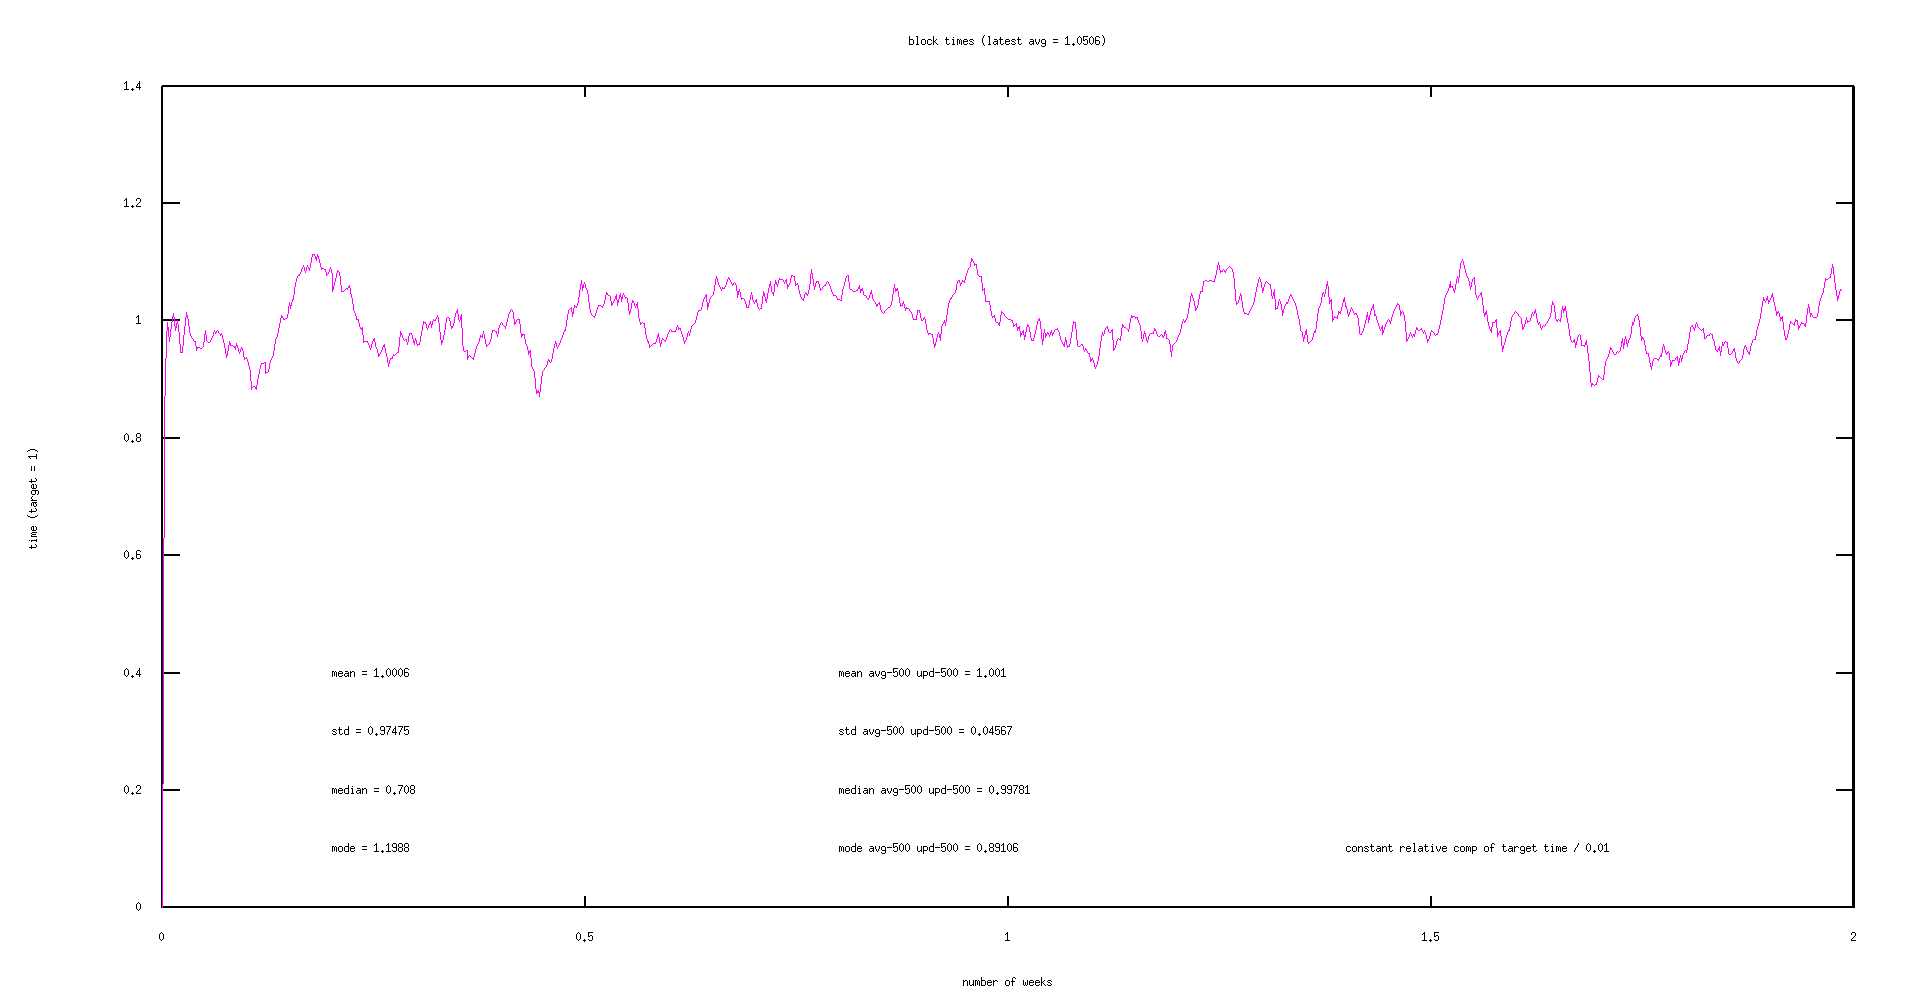
\includegraphics[width=14cm]{SimulationGraphs/simulation_avg-500_upd-500_Pcontroller.png}

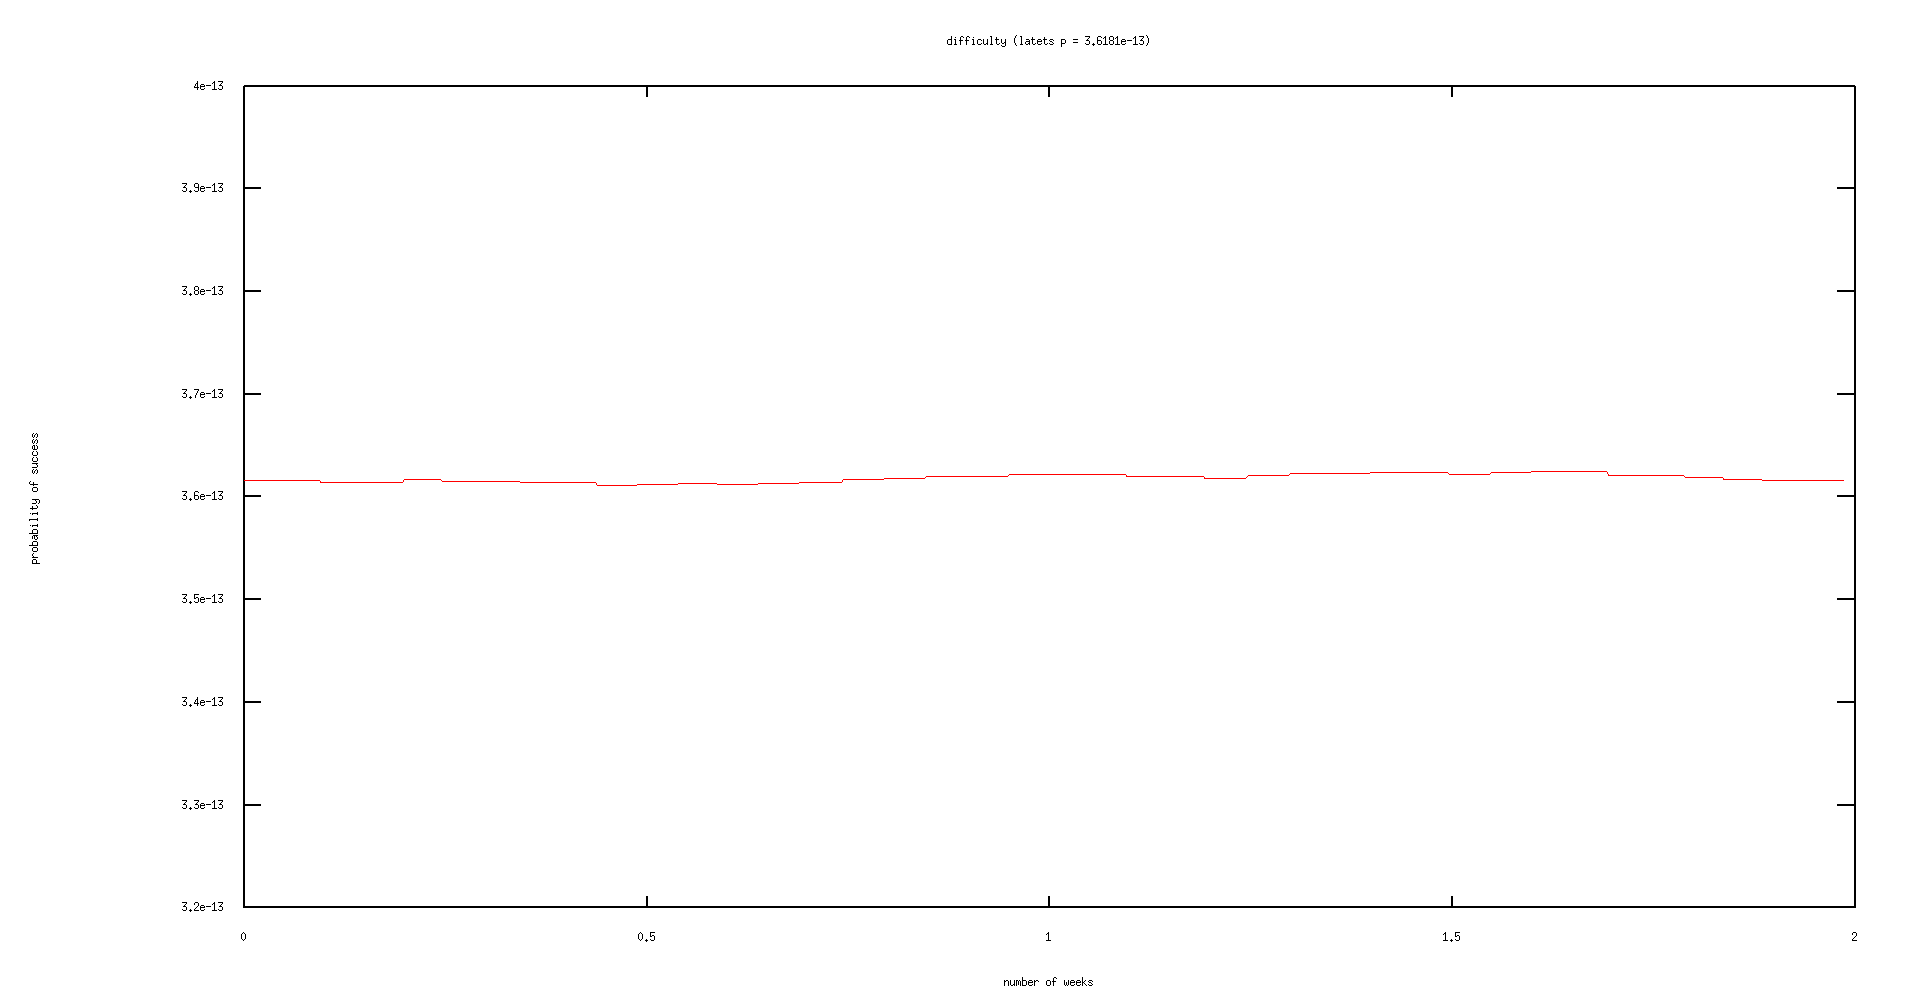
\includegraphics[width=14cm]{SimulationGraphs/simulation_avg-500_upd-500_Pcontroller_diff.png}

Tuning this to perform adequately over the full range of processor speeds is at best tricky and time-consuming, and might not actually be possible.

\newpage

A more sophisticated controller, which is potentially more stable over a larger range of network sizes, is the PID controller (see wikipedia). The update algorithm then takes the form:

\begin{verbatim}
last_error := error
this_error := 1 - (timestamp(n-1) - timestamp(n-500)) / (500 * 60)

integral := integral + this_error

derivative := this_error - last_error

K_p := 10^7;
K_i := 5.45 * 10^3;
K_d := 10^-3;

update := K_p * error + K_i * integral + K_d * derivative
difficulty(n) := difficulty(n-1) + update
\end{verbatim}

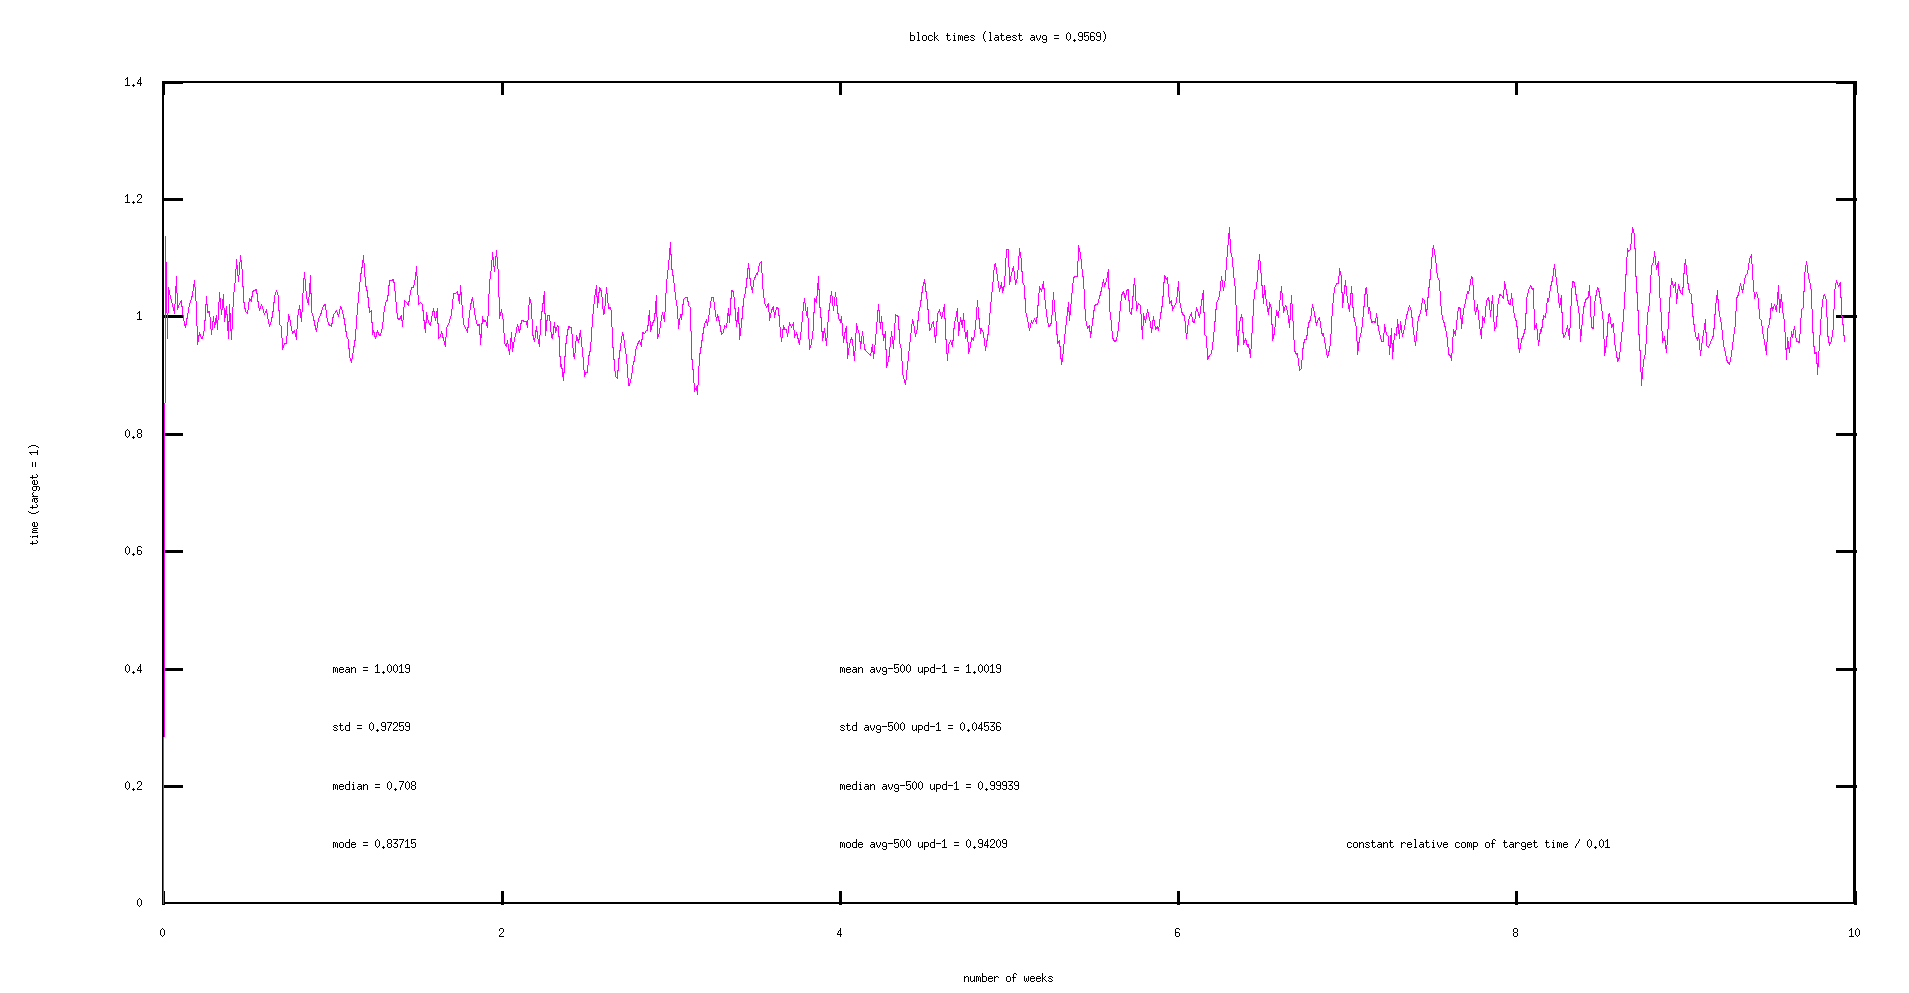
\includegraphics[width=14cm]{SimulationGraphs/simulation_avg-500_upd-1_PID.png}

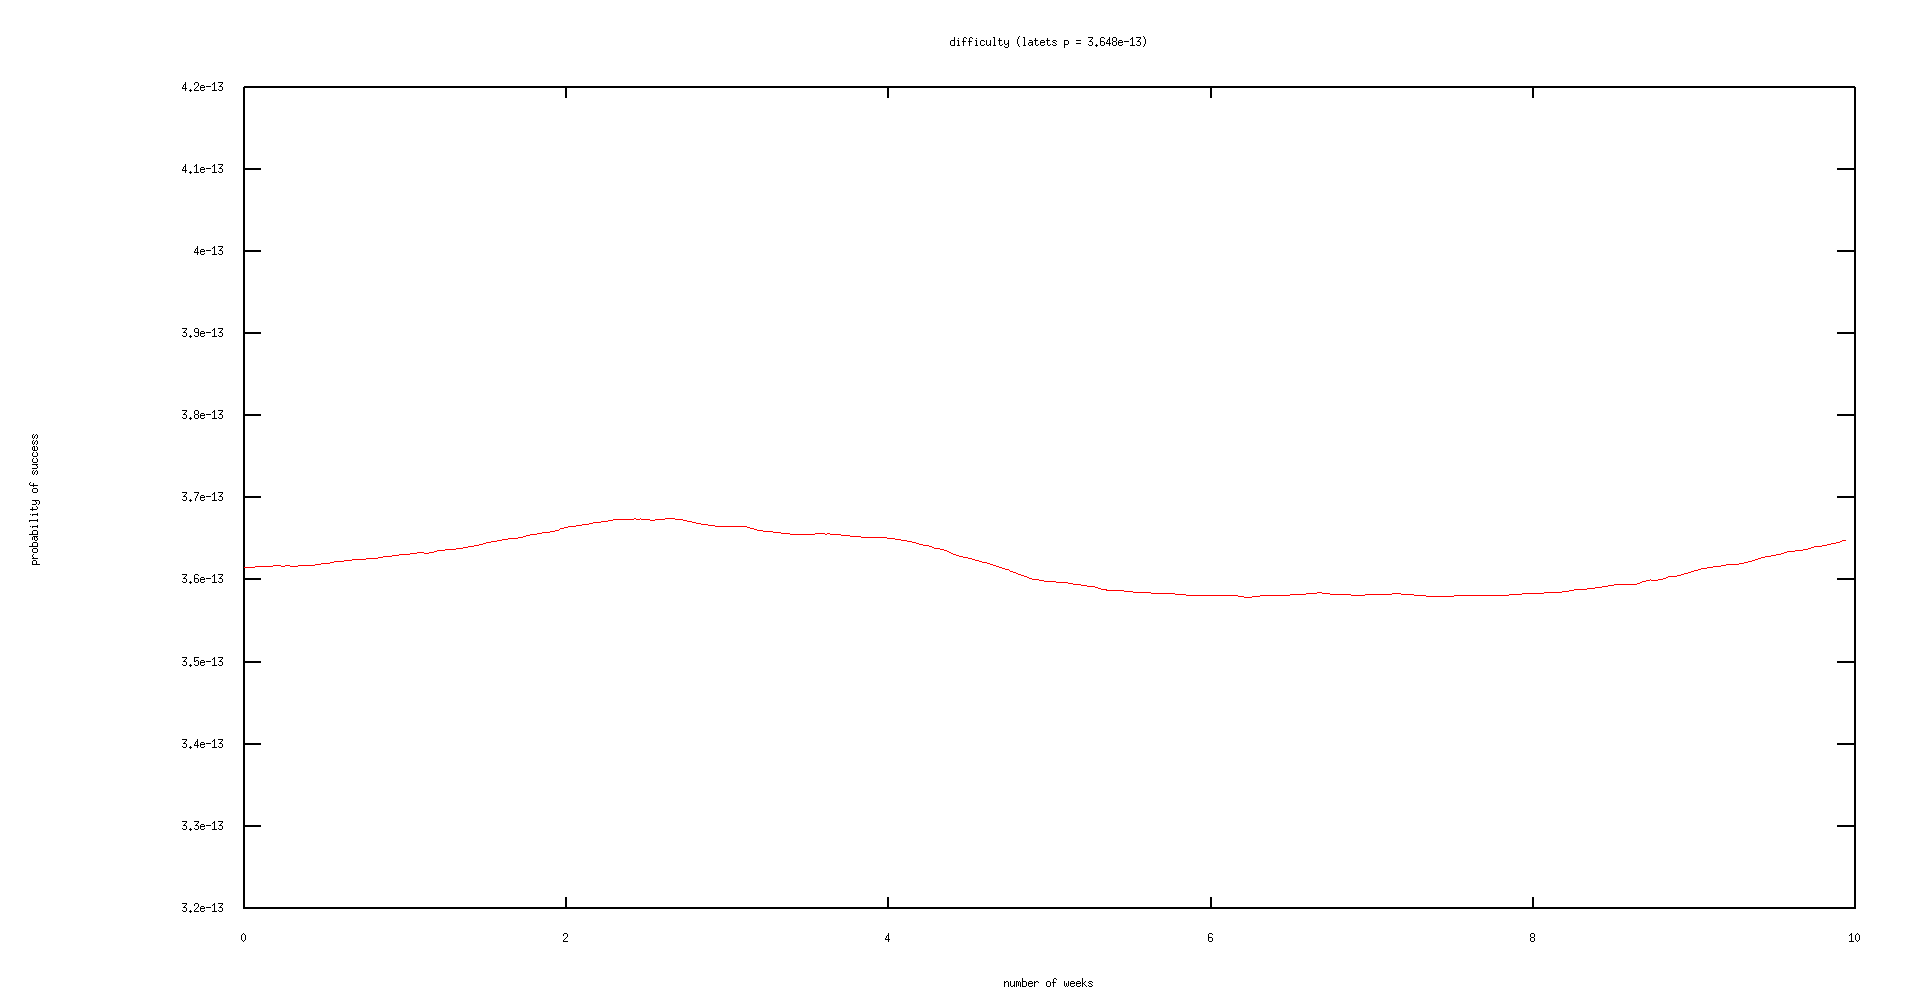
\includegraphics[width=14cm]{SimulationGraphs/simulation_avg-500_upd-1_PID_diff.png}

The PID controller offers the potential for good stability in steady state as well fast response to changes in node processor profiles. Many more simulations would need to be run to get anything close to optimal parameters. Although far from optimal, initial tests suggest the above parameters are an adequate start.

\newpage

For comparison, this is what steady state looks like with an single optimized difficulty setting:
\begin{center}
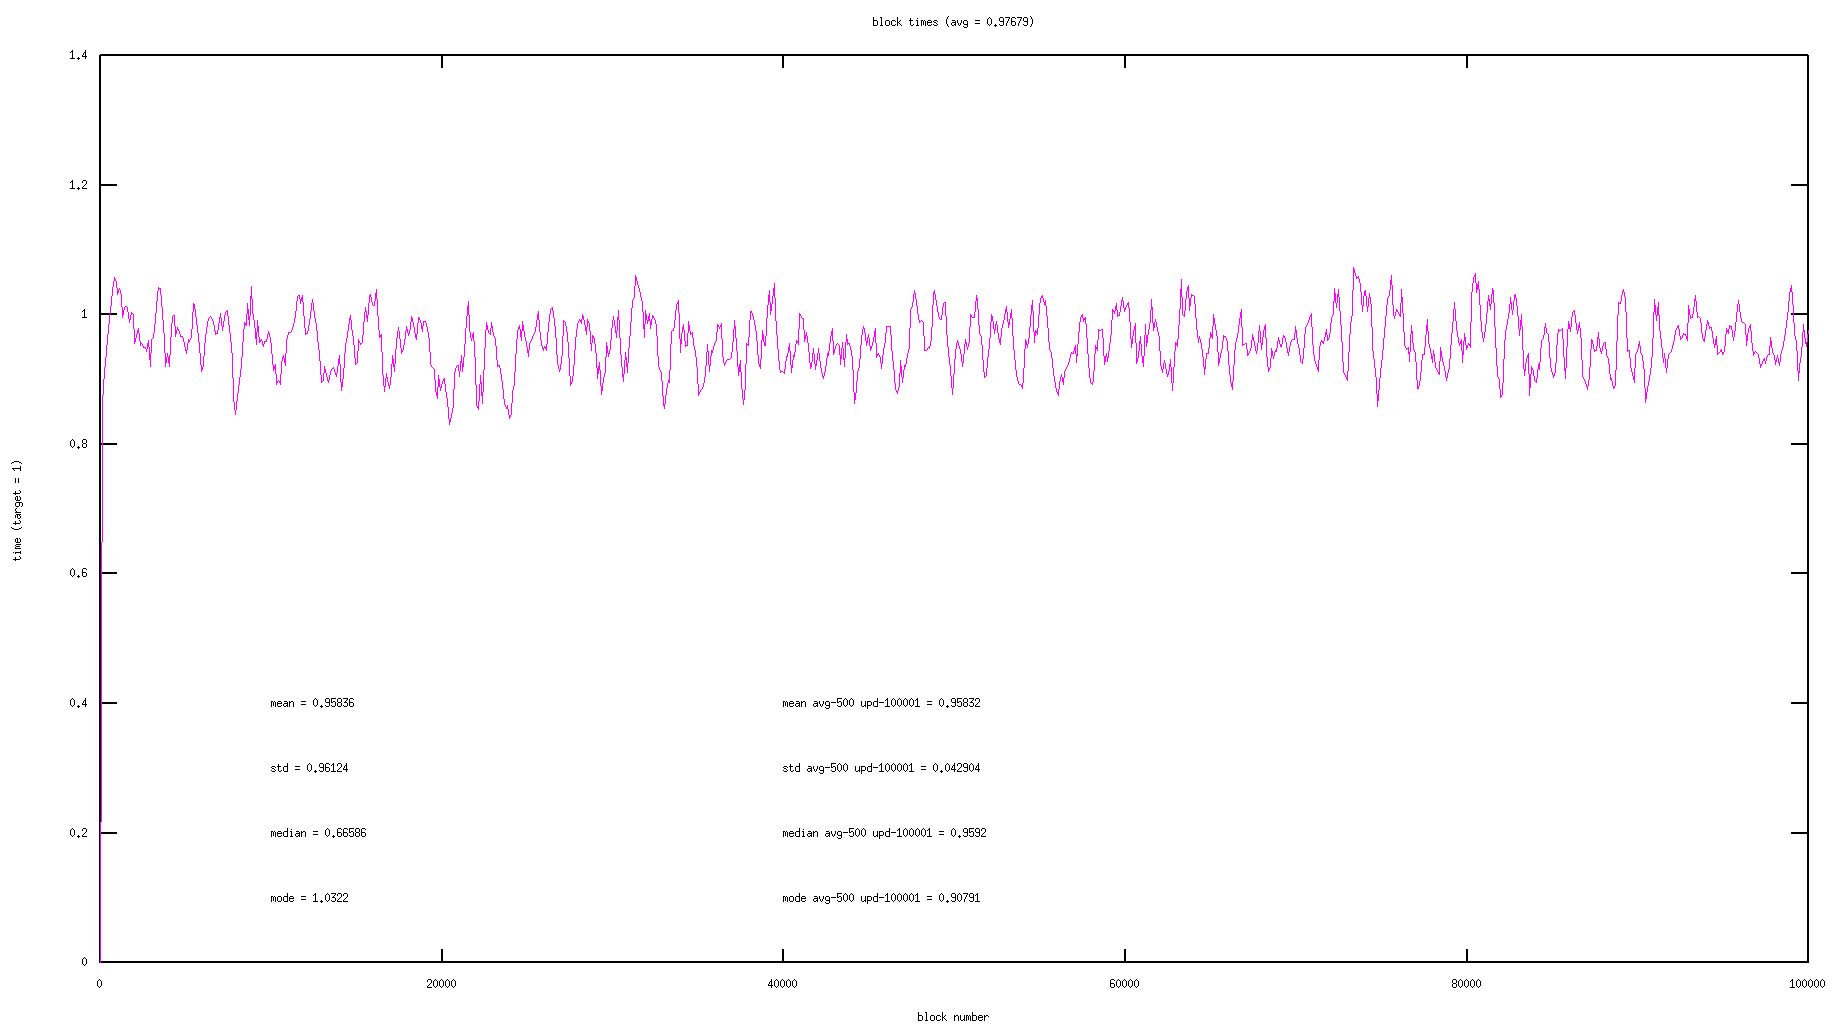
\includegraphics[width=12cm]{SimulationGraphs/simulation_avg-500_upd-none.png}
\end{center}

\section*{Other Approaches}
	Another alternative is to model the difficulty transfer function so we can guess the difficulty required to achieve the target block-time given the current distribution of node computation power. Determining that is way beyond the scope or ability of the system, so there's little point in pursuing that strategy. 
	
	Finally, we could copy bitcoin. As I understand it, bitcoin sets the difficultly every 2000 blocks (roughly every 2 weeks) using the following update algorithm:
	
\begin{verbatim}
difficultly(0) := 1

if mod(n, 2015) = 0
{
    average_time := (timestamp(n-1) - timestamp(n-2015)) / (2015 * 60)
    update := 10 / average_time
	
    if update > 4
        update := 4
    else if update < 0.25
        update := 0.25
        
    difficulty(n) := difficulty(n-1) * update 
}
else
{
    difficulty(n) := difficulty(n-1)
}
\end{verbatim}

\url{http://bitcoin.stackexchange.com/questions/5838/how-is-difficulty-calculated}

\newpage

If this is applied to Ethereum, the updates occuring every 2000 blocks will come up once every 1 day and 9 hours, which is fast enough, I reckon, although updates every 1000, or even 500 blocks seem not much less stable. While the steady-state updates jump around a little, the performance profile is perfectly adequate. The disadvantage of this update scheme is that it is purely reactive: the difficulty setting will always be behind the curve. However, updating every day will mean Ethereum won't be very far behind.

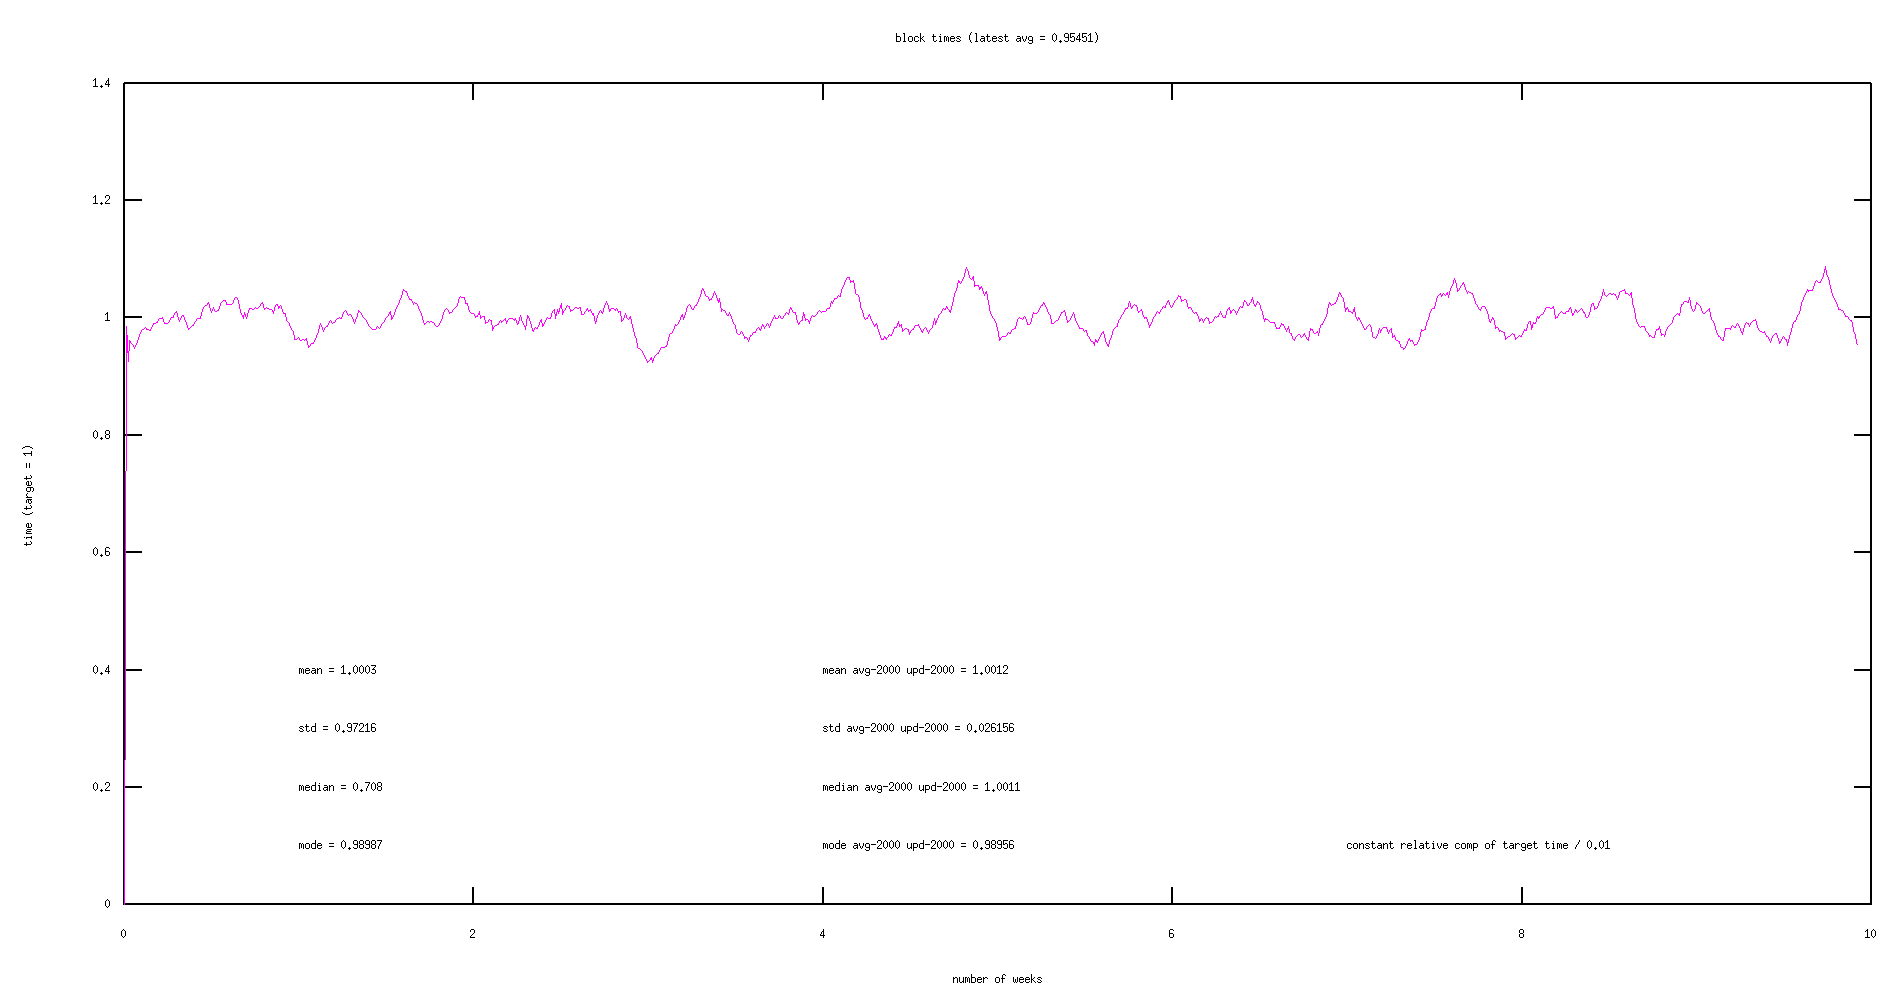
\includegraphics[width=14cm]{SimulationGraphs/simulation_avg-2000_upd-2000_btc.png}

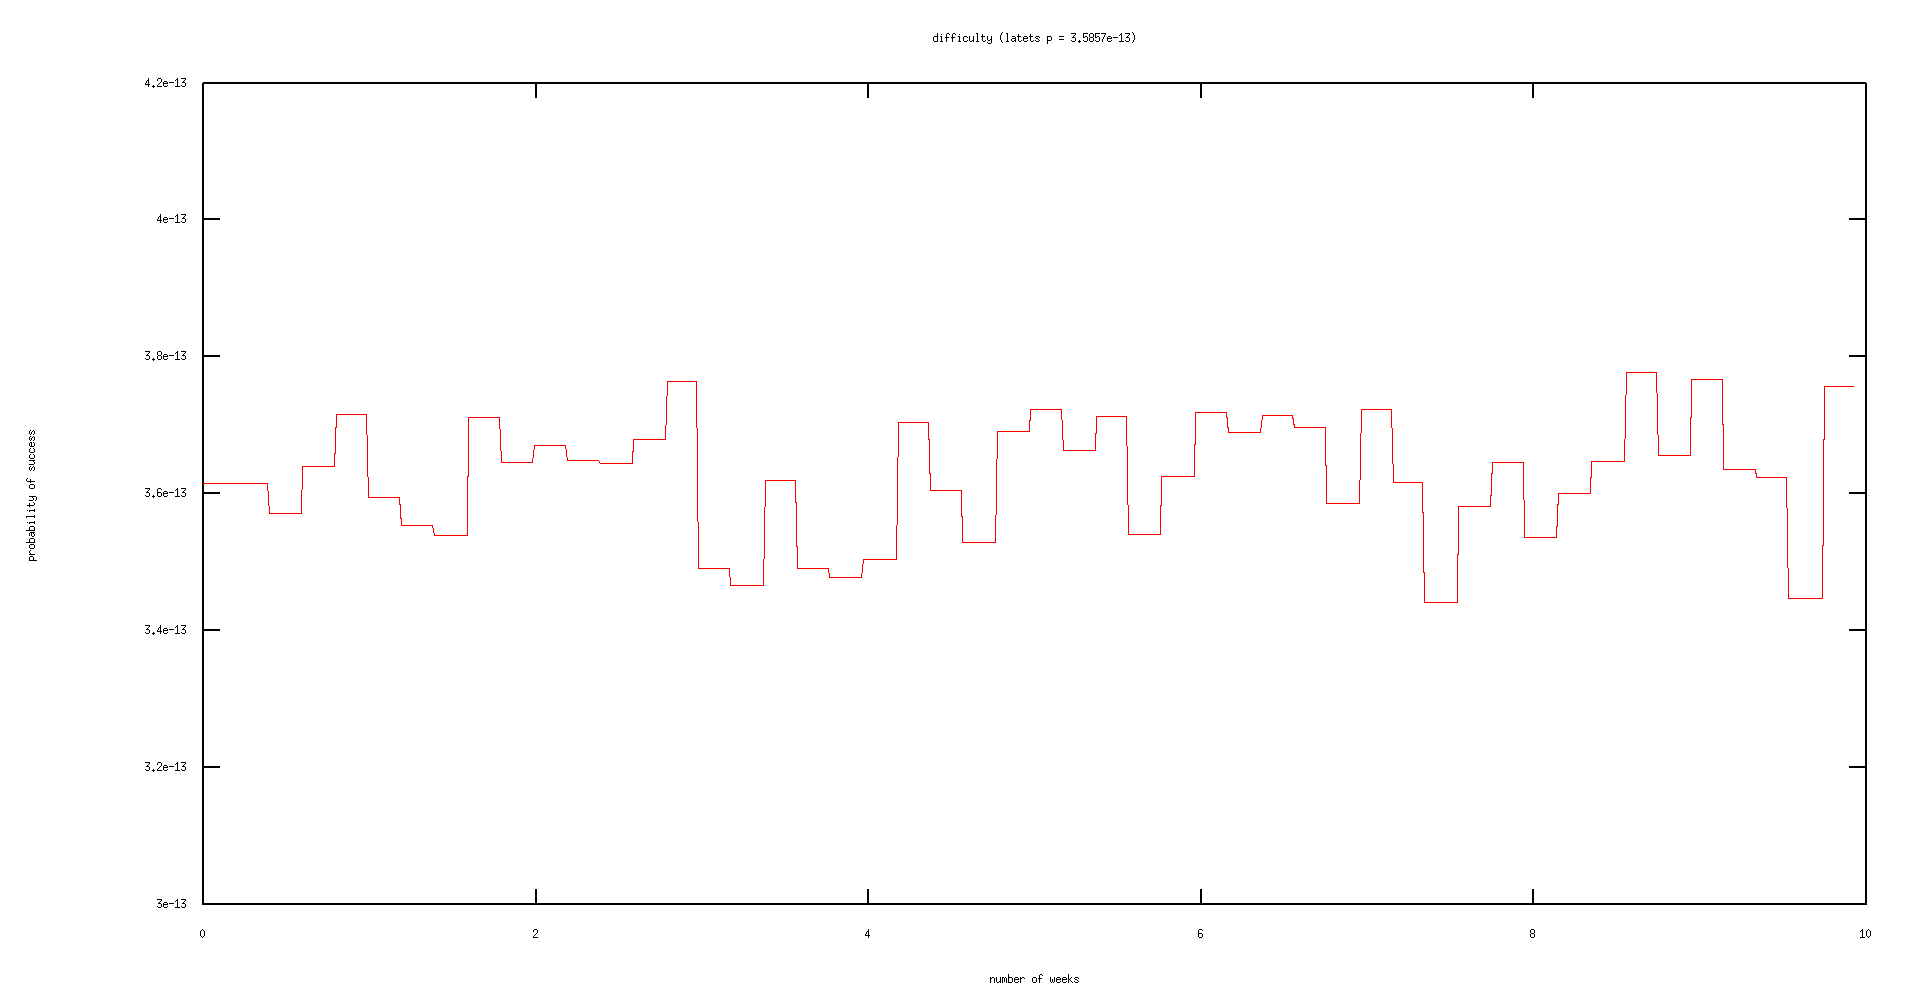
\includegraphics[width=14cm]{SimulationGraphs/simulation_avg-2000_upd-2000_btc_diff.png}



\end{document}